\section{Baseline Competitors}
To show the performance gain archived by our proposed solution in section \ref{sec:contribution} we use 2 baseline competitors.
The 2 competitors are chosen as they use simple and well known caching techniques. Both competitors take advantage of the optimal substructure property of the cached shortest path items.

\subsection{LRU}

LRU - Least Recently Used. This competitor uses the LRU cache replacement policy which gives each cache item a timestamp when it is added to the cache, and updates the timestamp if the cache item contributes to a cache hit. When a \spath query does not generate a cache hit, the new \spath will trigger a cache replacement. LRU simply throws out the cache item with the lowest timestamp and adds the new cache item with the current timestamp.

\subsection{FIFO}

FIFO - First In First Out. FIFO replaces, as the name suggests, the oldest cache item when a new \spath item is calculated and needs to be added to the cache. FIFO is the simplest of the suggested cache replacement policies.




\section{Contribution} \label{sec:contribution}

\subsection{Solution Proposals}

The techniques proposed here will each present how, and in what way, they can contribute to fulfilling the goals set out in section \ref{subsec:goals}.

All cache replacement techniques presented takes advantage of the optimal substructure property of shortest path, so all items in the \spath cache can also answer queries which only need a part of the shortest path.


\subsubsection{Cache Replacement Policies}

By using a cache a replacement policy, we try to directly shorten the total execution time by reducing the number of times the \spath algorithm has to be executed. 
The execution time is shortened every time we have a cache hit since the \spath algorithm\footnote{This can be any \spath algorithm, and we a just referring to the general set of \spath algorithms} does not need to run, and \spath algorithms usually are quite expensive in terms of the number of calculations and/or comparisons it needs to do to produce a result.


\paragraph{\osc}

\osc uses two scoring mechanisms which can both be added or multiplied to each other to assign each cache item a score. OSC does cache replacement based on the calculated score. If a new cache item get a lower score than any of the existing cache items it will not replace any existing cache items and will be discarded, if one or more items exist in the cache which have a lower score than some new candidate, then the item with the lowest score will be replaced.\ref{fig:advancedroutequery}

\ffh{write argument why to use + or * when calculating score.}

The scoring is done by summing up: the number of times a cache item has formed the basis of a cache hit; the number of times each node in cache item has been the source/target nodes in a query, or member of a query result. By taking the length of the \spath in a cache item and multiplying it on the previously calculated sum we get the full score.

\paragraph{Scoring Mechanism}

In \osc we use a scoring mechanism to rank the usefulness of cached items. Table \ref{tab:score} shows 3 queries ($i$) seen at different frequency and with different length. C(l) calculates the number of vertices visited when finding a shortest path with a \spath algorithm. Based on these numbers it is then possible to calculate the benefit of adding one of these \spath queries to the cache. E.g. Item 1 has higher frequency than item 2, but the saving of putting item 2 in cache is much higher:

item one cost: $11*100=1100$ and item two cost: $10*200=2000$. Assuming a cache hit cost $1$, then adding item one would save = $1100-(100+10*1)=990$, and item two would save $2000-(200+9*1)=1791$. the equation is: $(total\_cost\_without\_cache) - (cost\_of\_one\_Dijkstra\_run + (total\_runs-1 * cost\_of\_cache\_hit))$


\begin{table}
\begin{center}
\begin{tabular}{l |l |l |l}
i & item freq & item length & C(l) \\
1 & 11 & 10 & 100 \\
2 & 10 & 15 & 200 \\
3 & 2 & 15 & 2000 \\
\end{tabular}
\end{center}
\caption{\spath queries ($i$), their frequency, length, and cost of calculating result($C(l)$)}
\label{tab:score}
\end{table}


\ffh{C(l): modify Dijkstra implementation to return this number}



\acresetall
\subsubsection{\sps}

If space consumption is a very high priority then \sps is one option to alleviate the problem. \sps changes the cache structure from $n_1, ... , n_n$ to $CI_{k\left[s-node\right]},CI_{k\left[e-node\right]}, n_{e-node+1}, ... , n_n$.\footnote{This example only shows how to share something in the front of an item, though adding them after or in the middel does not matter.}
I.e. including the start-/end-node of a range from another cache item. The advantage of doing this is a, possibly large, reduction in the space requirements for the cache. Maintaining such a cache would be quite expensive in terms of computation when changes occur, though the space saving would allow for more cache items which again would reduce the total running time. We will later show wether this overhead can really be offset by the additional number of cache items which would fit into the cache.


how does it work?
what goal does it fulfill?
how does it fulfill the goal?
\subsubsection{Partitioning Map}

partitioning of map into large region to quickly be able to discard items in the cache, leading to less work when trying to find a cache hit. By discarding possible \spath cache candidates early we may save some time and computations.


\subsubsection{Cache structures}

\ffh{flesh out, add figures to clarify the difference}
\begin{itemize}
\item array, no utilization of optimal substructure property of \spath items
\item array, utilizing optimal substructure property of \spath items
\item 2D array, to more quickly (and cheaper) identify cache hits (expensive to maintain)
\end{itemize}


% % % % % % % % \subsection{Text and ideas which may still be useful (not part of paper)}
% % % % % % % % 
% % % % % % % % \ffh{need to focus on arguing about archiving lowest possible run time, do not connect to strongly with one map/graph, argue independently of map/graph that cost model and methods will be good.}
% % % % % % % % 
% % % % % % % % 
% % % % % % % % 
% % % % % % % % Figure \ref{fig:simplemap} shows a simple graph which we will use as our map and figure \ref{fig:simpleroutequery} shows the simple scenario in which a user (fig. \ref{fig:simpleroutequery}A) issues a route-planning query from 1 to 4 (fig. \ref{fig:simpleroutequery})  to an online route-planning server with a build in cache (fig. \ref{fig:simpleroutequery}B).
% % % % % % % % 
% % % % % % % % \subsubsection{Baseline}\label{baselinemethod}
% % % % % % % % \ffh{no longer used, but might be okay to use some parts for some motivation of why we want to do caching, or an intro to how the system works.}
% % % % % % % % The strait forward baseline solution is illustrated in figure \ref{fig:simpleroutequery}B. The idea is a server side shortest path cache which will store each query result in the cache and only consider exact query matches as cache hits, and to only use a simple cache policy such as LRU or FIFO.
% % % % % % % % The advantage of this solution is clear: it is simple and easily implemented. 
% % % % % % % % This simplicity is however obviously also it's main disadvantage, as it is too simple and very inefficient in terms of the utility the cache provides. Using items in the cache only when there is an exact match makes it exceedingly unlikely to get a cache hit due to the nature of route planning (many people share parts of routes, but few the same start and end points) and the sheer number of start-/end-point combinations possible.
% % % % % % % % 
% % % % % % % % \begin{figure}
% % % % % % % %   \center
% % % % % % % % 	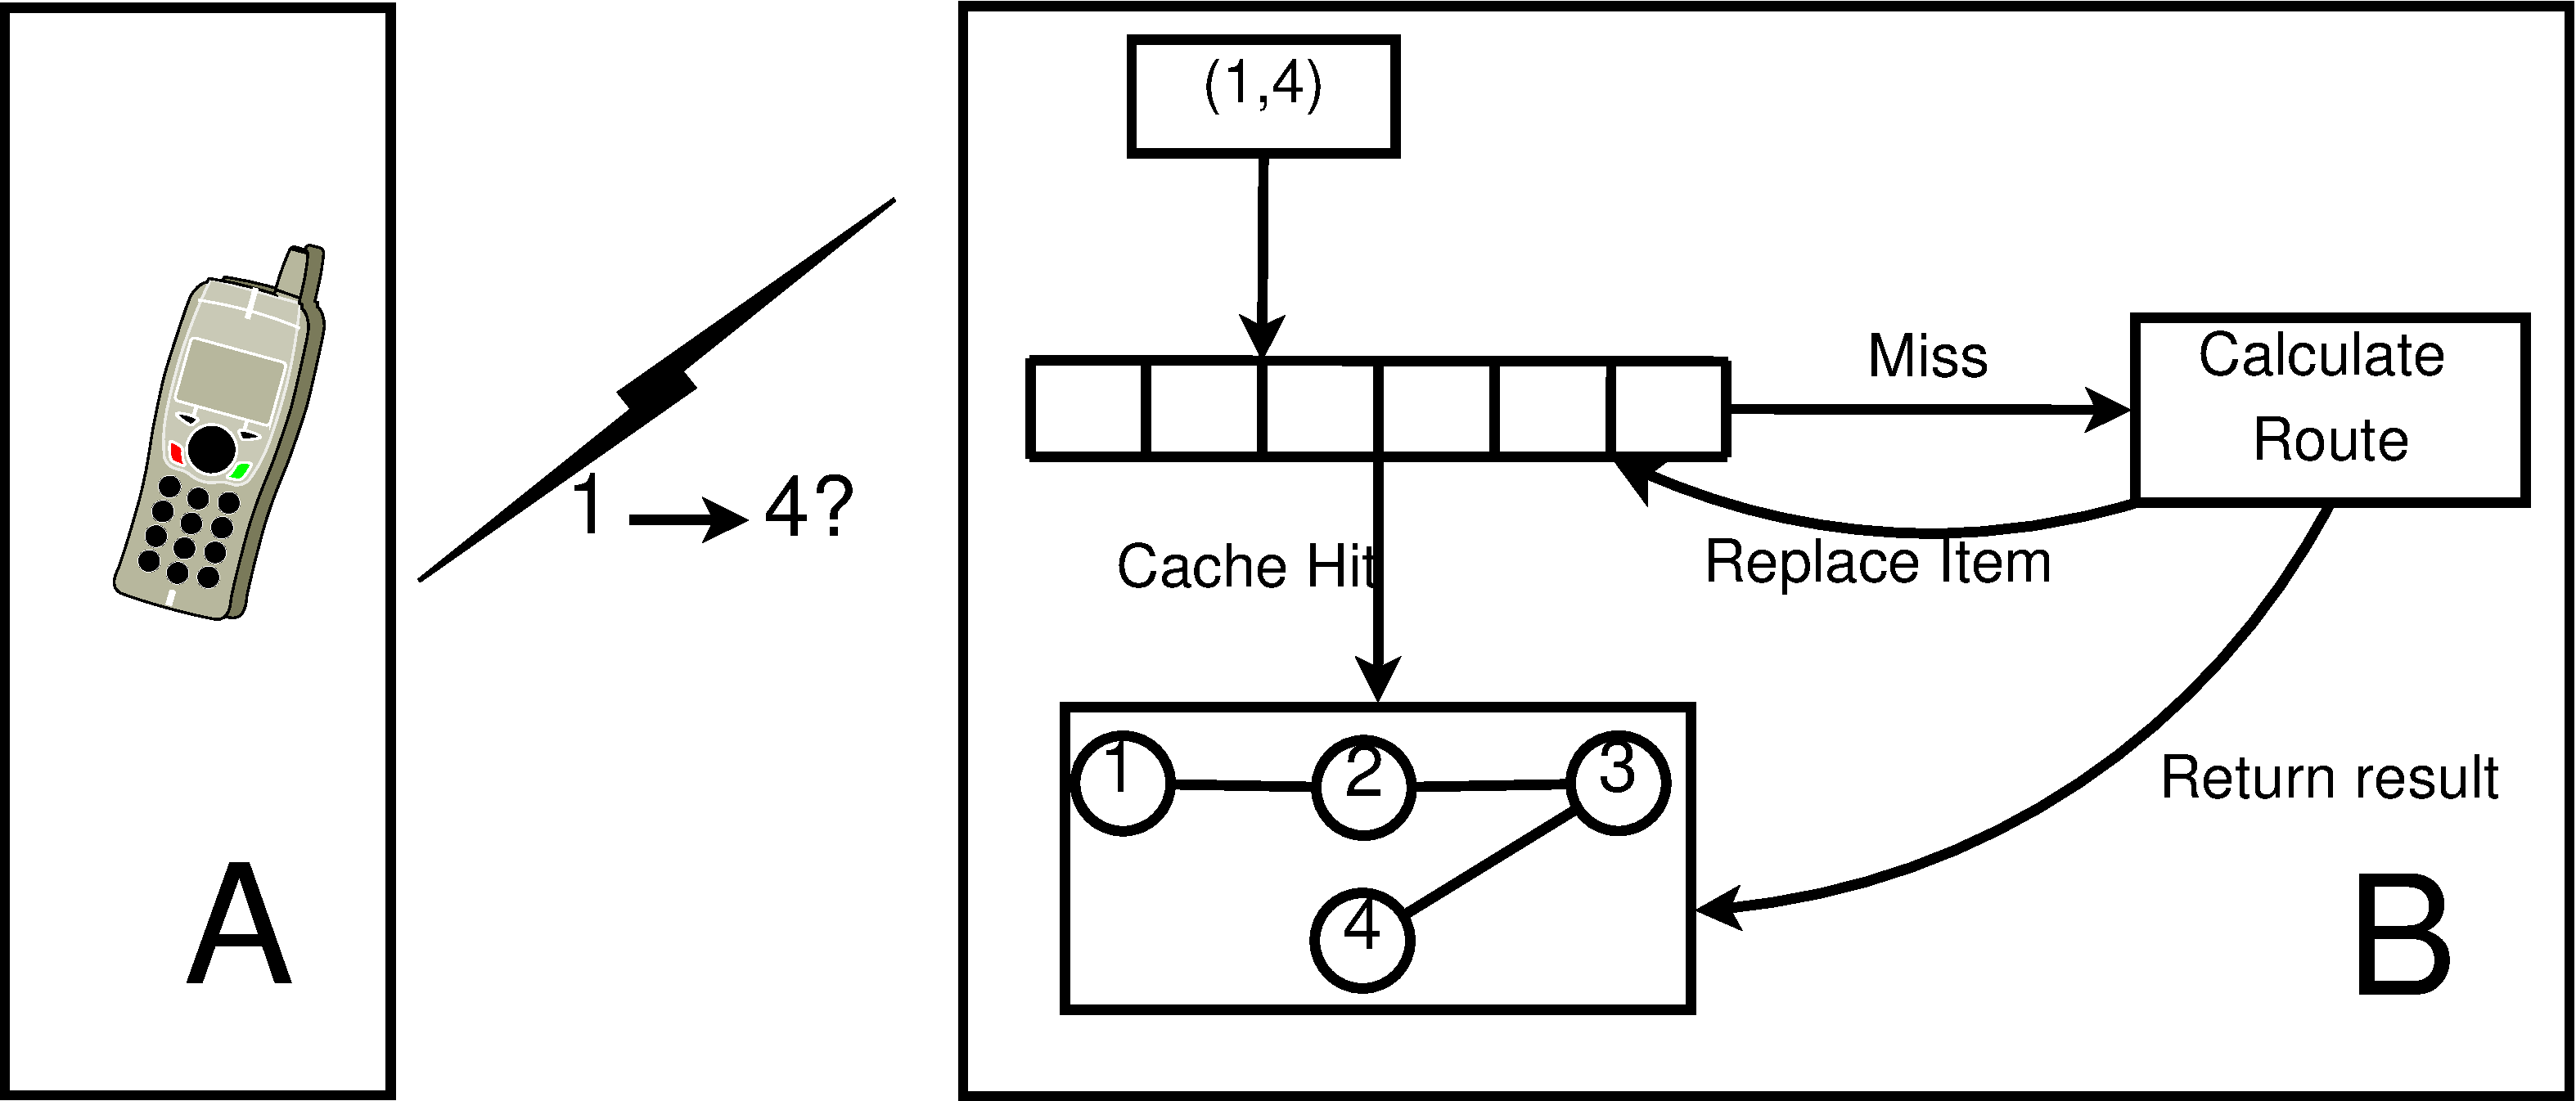
\includegraphics[width=0.5\textwidth]{figures/simpleroutequery.pdf}
% % % % % % % % 	\caption{simple graph}
% % % % % % % %   \label{fig:simpleroutequery}
% % % % % % % % \end{figure}
% % % % % % % % 
% % % % % % % % \subsubsection{Improved Baseline}\label{baselinemethodimp}
% % % % % % % % \ffh{no longer used, but might be okay to use some parts for some motivation of why we want to do caching, or an intro to how the system works.}
% % % % % % % % One way to possible increase the utility of a naive cache as proposed in \ref{baselinemethod} would be to exploit the \textit{optimal substructure property}\cite{introalg} of the cache items.
% % % % % % % % There is a significant increase in cache hits to be expected by utilizing the optimal substructure of shortest path cache items since it is unlikely many people will plan a route from/to the same place, but it is very likely that some sub-parts will be shared among users, and some users' full path laying within a longer path already calculated. The idea is illustrated in figure \ref{fig:cacheQueries} where the baseline method would be able to answer query Q1 from the cache, but not Q2. It is this specific disadvantage which ImpBaseline addresses and ImpBaseline can therefor answer both Q1 and Q2 from the cache since the result of Q2 now exist as a solution to a subpath of cache item C3.
% % % % % % % % Doing this adds a need for additional computational resources \ffh{how many resources?} required to examine the substructure of each  cached shortest path search result. It is currently not known if doing this is worth the effort, compared to just calculating the route, possibly multiple times.
% % % % % % % % 
% % % % % % % % \begin{figure}
% % % % % % % %   \center
% % % % % % % % 	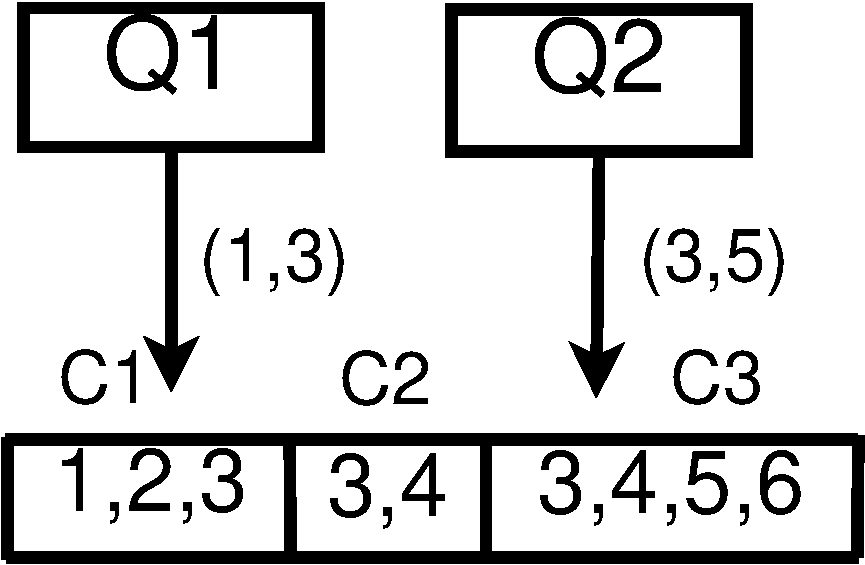
\includegraphics[width=0.25\textwidth]{figures/cacheQueries.pdf}
% % % % % % % % 	\caption{Queries}
% % % % % % % %   \label{fig:cacheQueries}
% % % % % % % % \end{figure}
% % % % % % % % 
% % % % % % % % 
% % % % % % % % \subsubsection{SP Results - facts}
% % % % % % % % \ffh{just to remember what facts I have available}
% % % % % % % % \begin{itemize}
% % % % % % % % \item number of times each node in query has been relevant to: 
% % % % % % % % \begin{itemize}
% % % % % % % % \item a cache hit
% % % % % % % % \item a query result
% % % % % % % % \end{itemize}
% % % % % % % % \item number of times source/target -nodes has been used in a query
% % % % % % % % \item sub-paths which are popular in query results (connected nodes which all "`score high"')
% % % % % % % % \end{itemize}
% % % % % % % % 
% % % % % % % % 
% % % % % % % % ---------------
% % % % % % % % 
% % % % % % % % \begin{deff}
% % % % % % % % A \textbf{SP Cache element} is a list $\left(v_s,v_{1},...,v_t\right)$ of vertices where $v_s/v_t$ are the start/end vertices of the list. $v_s$ is connected with $v_t$ by a shortest path defined by the vertices between $v_s$ and $v_t$ in the list.
% % % % % % % % \end{deff}
% % % % % % % % 
% % % % % % % % The cache is a set $\left\{SP_0,...,SP_n\right\}$ of SP cache elements. 
% % % % % % % % 
% % % % % % % % \begin{deff}
% % % % % % % % Cache replacement: Given two otherwise equal SP results, i.e. having the same length and having the same \textbf{value} (by some scoring mechanism defined for cache replacement) the SP result already in the cache will stay in the cache.
% % % % % % % % \end{deff}
% % % % % % % % 
% % % % % % % % 
% % % % % % % % \ffh{what other SSSP algorithms might be useful in comparing speed difference between cache and SP calculation?}
% % % % % % % % 
% % % % % % % % \ffh{Argue that since storing map data is cheap (little space required) but calculating SP is very expensive, then using the same, or more, space for cache than used for map data makes sense.}
% % % % % % % % 
% % % % % % % % ------------------
% % % % % % % % 
% % % % % % % % 
% % % % % % % % To initially identify basic weaknesses and strong points of our ideas we validate some of our simpler assumptions using a uniform random model(URM) together with a simple 'map',the graph in figure \ref{fig:simplemap}, enabling us to clearly reason about the advantages expected when using server side caching of \spath queries. By using the simple map (fig.\ref{fig:simplemap}) and a URM together with we can reason about the probabilities that a specific query will occur. Figure \ref{fig:queryprob} illustrates the number of queries possible for a map with 2,3, and 5 locations for figure \ref{fig:queryprob}A, \ref{fig:queryprob}B, and \ref{fig:queryprob}C respectively. Each line underneath each of the simple graphs represents two possible queries (A->B, B->A). The number of shortest-path queries possible on a tree-graph with n vertices is $n*(n-1)$. The probability of seeing any one query, $q_i$ is then $P(q_i | n) = (n*n-1)^{-1}$
% % % % % % % % 
% % % % % % % % \begin{figure}
% % % % % % % %   \center
% % % % % % % % 	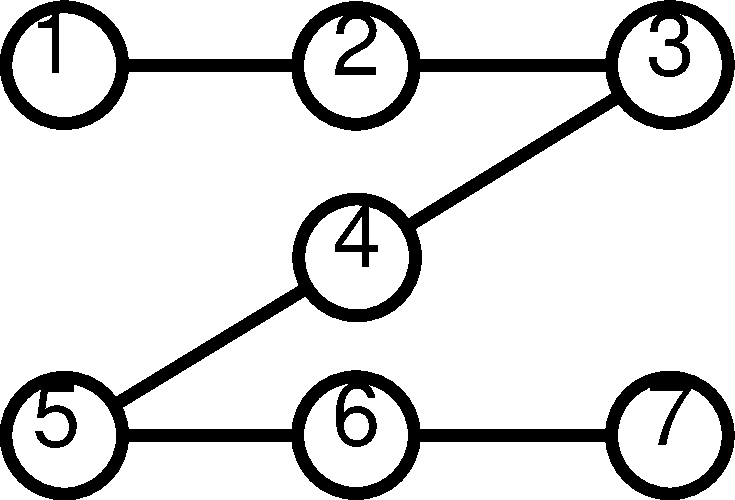
\includegraphics[width=0.25\textwidth]{figures/simpleMap.pdf}
% % % % % % % % 	\caption{Simple map}
% % % % % % % %   \label{fig:simplemap}
% % % % % % % % \end{figure}
% % % % % % % % 
% % % % % % % % \begin{figure}
% % % % % % % %   \center
% % % % % % % % 	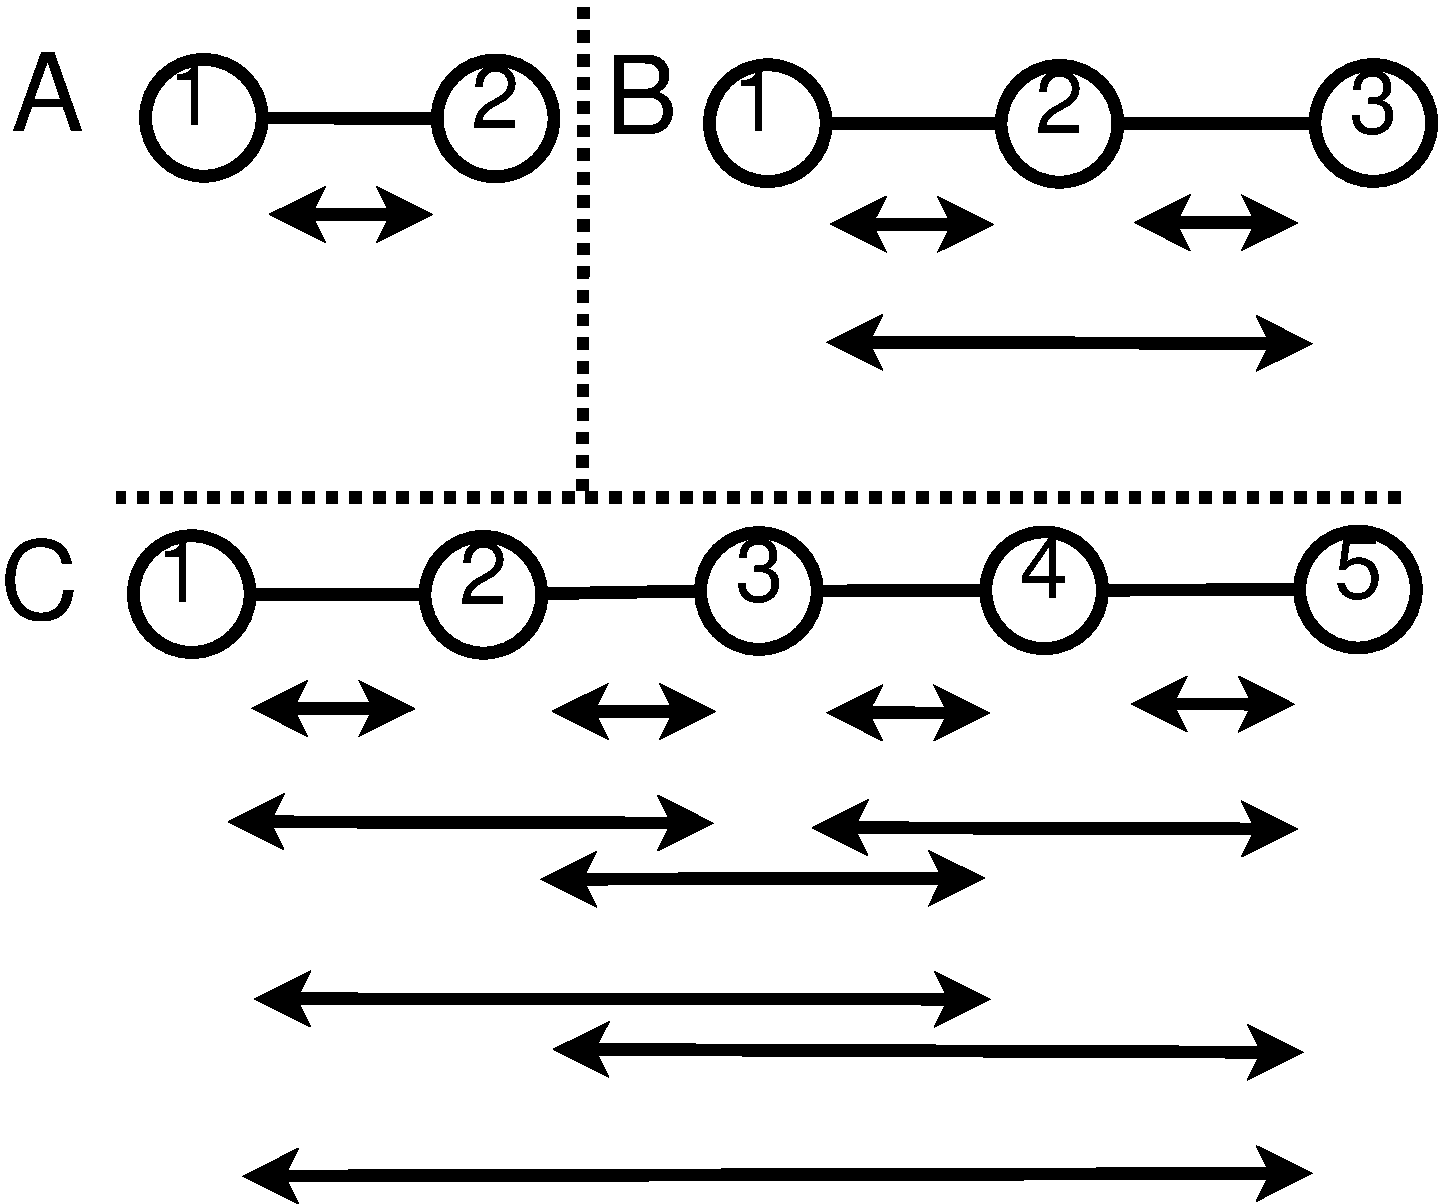
\includegraphics[width=0.25\textwidth]{figures/queryprob.pdf}
% % % % % % % % 	\caption{Number of queries possible}
% % % % % % % %   \label{fig:queryprob}
% % % % % % % % \end{figure}
% % % % % % % % 


% \section{Contribution} \label{sec:contribution}
% 
% We first introduce the motivation for what we want to protect, and what possible privacy leaks we foresee as being possible. Afterwards we present the protection schemes and types which the user can specify depending on how often a \poi is sensitive. Secondly we describe the privacy profile and the parameters the user can adjust. 
% %In table \ref{tab:poiclass1} we lists the different \poi classifications
% 
% \subsection{Motivation}
% %what privacy attacks do we want to prevent?
% %what privacy leaks could happen?
% The main goal of our proposed framework is to make sure that after we have applied users privacy profiles and removed any unique identifiers in the set of trajectories, an attacker can't tie a user to a unique trajectory. Additionally we want to prevent an adversary from determining if a user has \textit{visited} or \textit{been near} a sensitive \poins. Having visited or been near a sensitive \poi are two separate cases; in the former we just have to ensure that it can not be determined that a user has stopped at a \poins. In the latter case we have to hide that the user has been in the area at all. 
% 
% Assuming that an attacker would always have access to the yellow pages, or an equivalent there of, there still exist only two categories of attacks which in some circumstances can cause the privacy of a user to be breached,  the first being an attacker knowing of one point visited by a user along a trajectory, the second being the attacker knowing of the location of a user at 2 or more points on a trajectory.
% A more in dept explanation of these attacks and what the information an attacker could gain is presented in section \ref{subsec:attack}.
% 
% \begin{figure}
%   \center
% 	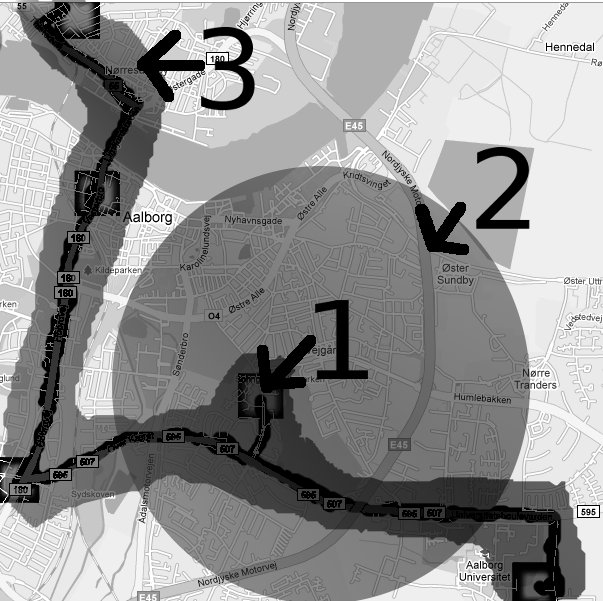
\includegraphics[width=0.2\textwidth]{figures/poitypes.jpeg}
% 	\caption{\poi categories. 1. Point, 2. Area, 3. Trajectory}
%   \label{fig:poiCategories}
% \end{figure}
% 
% 
% When users specify \pois they falls into three general categories, illustrated in figure \ref{fig:poiCategories}. The first category is a single spatial point on a map like e.g. a clinic or their place of occupation (Fig. \ref{fig:poiCategories}, [1]). The second category \pois is a sensitive area like e.g a park or neighborhood (Fig. \ref{fig:poiCategories}, [2]). The last category of \pois are routes or trajectories (Fig. \ref{fig:poiCategories}, [3]). 
% 
% When the user specify one of the three categories of \poisns, he is first specifying $p_{cover}$, a region (Fig.~\ref{fig:poiCategories}, [2,3]) or point (Fig.~\ref{fig:poiCategories}, [1]), which is translated to $p_{edges}$ a set of full and partial edges in the road network which is contained or intersecting with the region or point specified. After specifying $p_{cover}$ the user specifies the sensitivity by giving both a spatial and a temporal sensitivity value. With this we have definition~\ref{def:poi}.
% 
% \begin{deff}[\poins] \label{def:poi}
% A \poi $p$ is a tuple $(p_{edges}, d_s, d_t, class)$ where $p_{edges}$ is the set of tuples $\{(e, e_{from}, e_{to} | 0 \leq e_{from} < e_{to} \leq e_{length})\}$ which is sensitive. 
% $e \in \mathbf{E}$ and $e_{from}, e_{to}, e_{length} \in \mathbb{R}$. 
% $e_{from}/e_{to}$ specifies on $e$ the start-/end-location covered by $p_{cover}$. If $e$ is fully included in $p_{cover}$, $e_{from}/e_{to}$ is equal to $0/p_{length}$.
% $d_s, d_t, class \in \mathbb{N}$ is respectively the spatial sensitivity, the temporal sensitivity, and the \poi classification (Table~\ref{tab:poiclass1}).
% \end{deff}
% 
% Our approach makes a trade off between the data quality of the published data and the degree of anonymization on the provided in the dataset. This trade off will be a parameter controlled by the service provider. If the service provider prioritize data integrity to high and thereby sacrifice user privacy, an adversary would have a higher chance of breaking user privacy, i.e. connect a specific user to a trajectory.
% 
% When a user specifies that a particular point, area, or trajectory is sensitive to him, we want him to visually draw the sensitive part ($p_{cover}$) and afterwards indicate how important it is to the user not to be identified as having been in the area($d_s$), as well as how important it is to hide $when$ he has been in the sensitive area ($d_t$). As the third thing we also want the user to choose a classification from a list of candidates (Table~\ref{tab:poiclass1}). The system will handle the how of the anonymizing in the way it finds most fit, without any user involvement. $d_s$ is specified as the number of other users a user $u$ want to be indistinguishable from, and $d_t$ is specified as the time period within which user $u$ does not want it to be known when exactly a trajectory was generated.
% 
% 
% \subsection{Protection Schemes}\label{subsec:schemes} %can also be ways for user to specify how poi's are sensitive
% We have devised three different schemes for the user to choose between, to ensure user privacy depending on how often a \poi is sensitive.  Each scheme allows for different optimizations when anonymizing the trajectory dataset. The first scheme is \ac{AS} which handles the \poi considered to always be sensitive. The second scheme is a special case of \ac{AS}, namely \ac{ASTI} handling the case where a \poi sensitivity is restricted by a recurring time period e.g. 8-9 pm Monday-Friday. The \ac{RS} scheme handles the cases where a \pois sensitivity is non-recurring. When specifying \poi sensitivity this classification is easily understandable for the user.
% 
% 
% \subsection{Protection Types}\label{subsec:protectiontypes}
% 
% We define three ways of achieving the user specified level of anonymization for a given \poins, two being special cases of the first. Before we list the protection types we need to define Temporal k-anonymity (\tanonns) for trajectories. This concept is the cornerstone in our approach which ensures that a user can neither be tied to a specific trajectory, nor be identified as having visited a sensitive location. As mentioned earlier there are only two general attacks which might allow the attacker to gain more knowledge about a user than was polished in the anonymized dataset. These attacks are in all scenarios rendered useless when \tanon is applied no edge uniquely identifying any user will ever be published (e.g. a road to a private resident).
% 
% 
% 
% 
% \tanon depends on four parameters: $\mathbf{T}, p_{edges}, TP,\text{ and } t$. $\mathbf{T}$ is a set of trajectories. $p_{edges}$ is the set of edges covering a sensitive region of a trajectory in $\mathbf{T}$. $TP$ is a time period and $t$ is the number of trajectories where we want sub-trajectories covered by $p_{edges}$ to be spatially and temporal indistinguishable from each other when \tanon is fulfilled. 
% In order for some set of trajectories to fulfill \tanon they need to be spatially and temporally indistinguishable at the edges covered by $p_{edges}$, and additionally for each timestamp of a trajectory in the set, the timestamps of all others in the set needs to lie within $TP$
% 
% % \begin{deff}[\tanonns]
% % \label{def:tanon}
% % Given $\mathbf{T}$, the set of trajectories, and a \poi $p$. 
% % Let $\Gamma \subseteq \mathbf{T}$, be the set of all trajectories which subtrajectories intersect with $p_{edges}$ and lies within a time period $\mathbf{TP}$. $\Gamma$ is said to satisfy \tanon with respect to $\mathbf{TP}$ and a subtrajectory $s \in p_{edges}$ iff it contains at least $t-1$ other trajectories from $\mathbf{T}$ with sub-trajectories laying within $\mathbf{TP}$.
% % \end{deff}
% 
% \begin{deff}[\tanonns]
% \label{def:tanon}
% Given $\mathbf{T}$, the set of trajectories and $p_{edges}$, the set of edges covering a sensitive part of trajectory $\gamma$. 
% Let $\Gamma \subseteq \mathbf{T}$ be all trajectories which subtrajectories intersect with $p_{edges}$. $\Gamma' \subseteq \Gamma$ be all trajectories where, for edges intersecting with $p_{edges}$, at each timestamp of $\gamma$ their timestamps lie within a time period $TP$ symmetric around the timestamp of $\gamma$.
% $\Gamma'$ is said to satisfy \tanon with respect to $TP$ and $\gamma$ iff $\Gamma$ contains at least $t-1$ other trajectories.
% \end{deff}
% 
% There are two special cases of \tanonns: $\left(t = 1, TP < \infty \right)$ and $\left(t > 1, TP = \infty\right)$. If $t=1$ and $TP < \infty $ then a single trajectory is hidden within a time period but no spatial anonymization will be performed. The second special case is if $t > 1$ and  $TP = \infty$, in this case no temporal anonymization will be performed as a time period of infinity signifies that no temporal obfuscation is wanted and we are instead dealing with pure \kanon for trajectories. Since these two special cases combined encompasses what \tanon is about, but perhaps individually more easily understood we will provide a short explanation of how they both work.
% 
% 
% \kanon for trajectories is similar to \tanonns, though it imposes no restrictions on the timestamps inclusion within time period and as such its definition is alike that of of \tanon.
% 
% \begin{deff}[\kanonns]
% \label{def:kanon}
% Given $\mathbf{T}$, the set of trajectories, and $p_{edges}$, the set of edges covering a sensitive part of trajectory $\gamma$. 
% Let $\Gamma \subseteq \mathbf{T}$ be all trajectories which subtrajectories intersect with $p_{edges}$. 
% $\Gamma$ is said to satisfy \tanon with respect to $\gamma$ iff $\Gamma$ contains at least $k-1$ other trajectories.
% \end{deff}
% 
% Using \kanon a users' trajectory $\gamma$ would be indistinguishable from $k-1$ other users at the part within $p_{edges}$. Using the roadnetwork in figure~\ref{fig:roadnetwork} as a reference user $u$ might go from A to E to get from work to home, but $u$ goes to the Hospital at D on the way home, and want to hide this fact. Using \kanon the system can find $k-1$ other similar trajectories from A-D and D-E to ensure that nobody can identify $u$ with greater certainty than $\frac{1}{k}$. i.e. if an adversary sees $u$ at some point while $u$ drives he would know the when and where of $u$ and be able to match that information with a set of trajectories in the anonymized trajectory dataset. The set of candidate trajectories will however be at least $k$ large.
% 
% % \begin{deff}[\kanonns]
% % \label{def:kanon}
% % Given $\mathbf{T}$, the set of trajectories, and a \poi $p$. 
% % Let $\Gamma \subseteq \mathbf{T}$, be the set of all trajectories which subtrajectories lie in $p_{edges}$. $\Gamma$ is said to satisfy \kanon with respect to a subtrajectory $s \in p_{edges}$ iff it contains at least $k-1$ other trajectories.
% % \end{deff}
% 
% \begin{figure}	
% 	  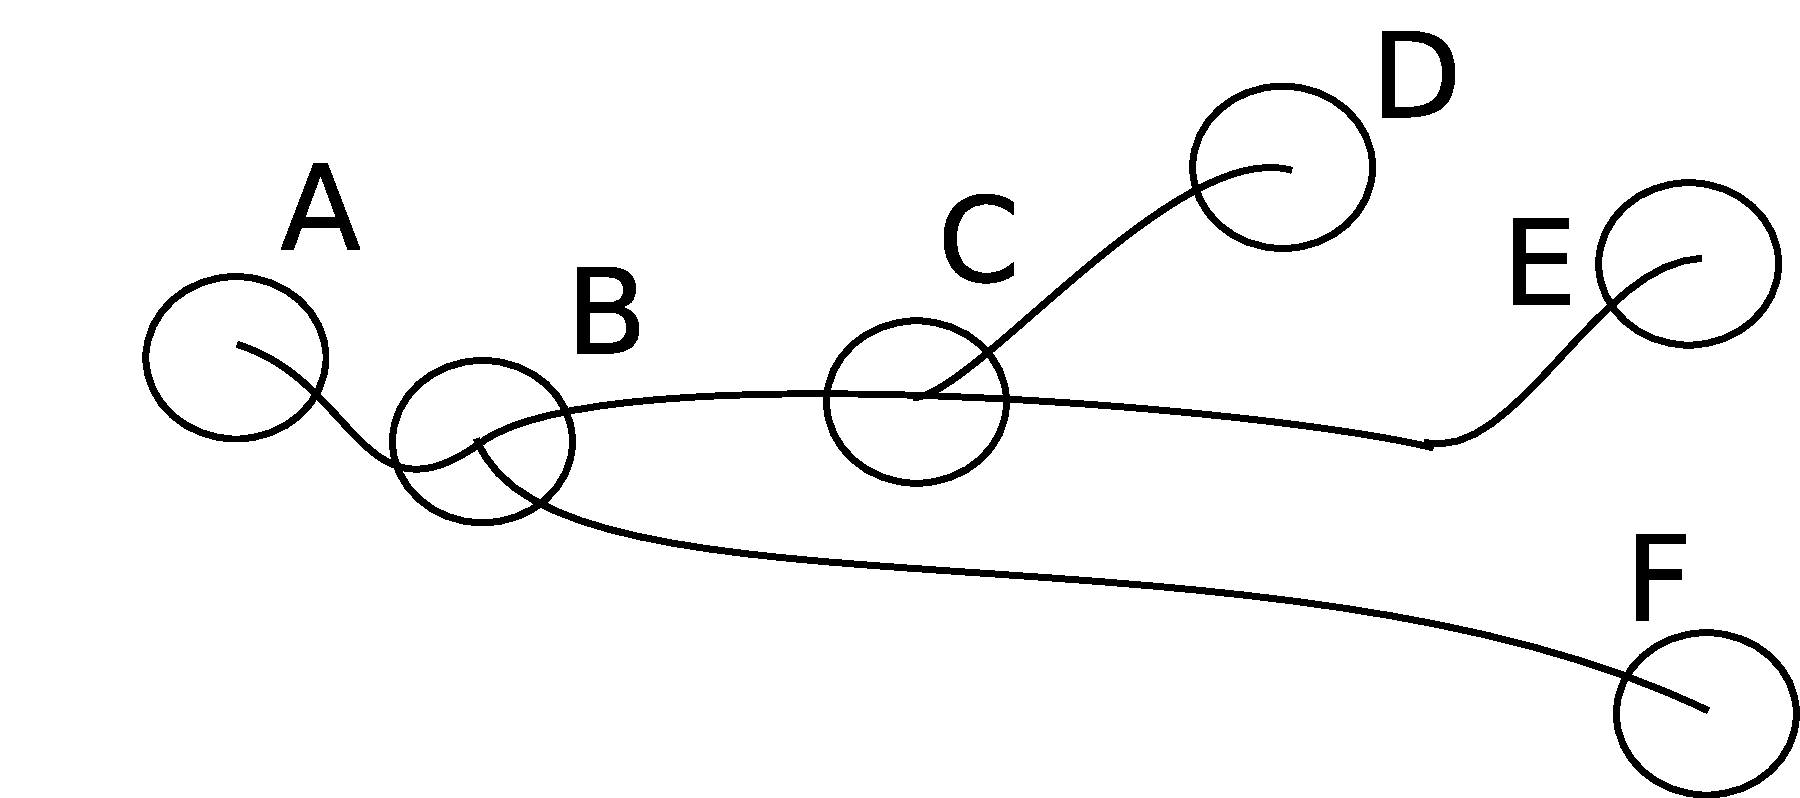
\includegraphics[width=0.25\textwidth]{figures/roads.pdf}
%        \caption{Simple road network}
%   \label{fig:roadnetwork}
% \end{figure}
% 
% 
% A {\it time period} works by manipulating a trajectory's timestamps which e.g. can be used to make it look like user $u$ never stopped at a specific location, or make it unclear when said stop was made. E.g. If a user $u$ decides to go to the Hospital, D, on his way home from work A-E (see Fig. \ref{fig:roadnetwork}) but he does not want it to be know when exactly $u$ has been there, or that he has been there at all. We can distribute out the time used at the hospital (Fig.~\ref{fig:adjustTrajec}A) so it looks like $u$ has been driving slower on remaining edges of the trajectory but never made a stop at the hospital (Fig.~\ref{fig:adjustTrajec}B).
% A user could also use a time period if he only cares about masking when he has been somewere i.e. if the trajectory taken was public knowledge or easily figured out, but the time of the trajectory was not (e.g. a money transport has to go to specific places, but when is unknown).
% 
% \tanon is conceptually a combination of \kanon and time period and as such an improvement on both. With \tanon it is thus much harder to figure out when and which edges $u$ actually visited, than if $u$ were using only \kanon or a time period. 
% A user is expected to almost always have specified a spatial and a temporal sensitivity and as such always be using \tanon when having his trajectories anonymized.
% 
% For our approach the mapping of input to \tanon is as follows: The set of trajectories $\mathbf{T}$ is still just that, $p_{edges}$ are $psr.p_{edges}$ from a \poi covering a sub-trajectory in $\gamma$. $t = psr.d_s$ and $TP = d_t$.
% 
% \tanon and the two special cases: \kanon and time period, represent different privacy needs and level of effectiveness when anonymizing. All of these types will work for all categories of \pois -  points, areas or full trajectories (see Fig. \ref{fig:poiCategories}). The aim is to prevent information leakage from the anonymized dataset via data correlation. A correlation attack could e.g. be if someone know when a user $u$ leaves from work and arrive at home, they could then figure out where else $u$ has been on the way from work. While examples are given for when a user would would use \tanonns, \kanonns, or time interval, the user is not meant to choose this directly, rather this will be inferred by our system from the temporal and spatial sensitivity specified for each \poins.
% %The correlation attack could also be done by looking at the timestamps on the trajectory before and after the sensitive region, since the attacker already know the route taken in the sensitive region he can then estimate the entire trajectory including approximate timestamps for the sensitive region.
% 
% 
% 
% 
% \subsection{\poi Classification}\label{subsec:protectpoitype}
% 
% \begin{table}
% 	\begin{center}
% 		\begin{tabular}{|c|}
% 			\hline
% 			\bf Classification	\\\hline
% 			Public Service Point	\\\hline
% 			House			\\\hline
% 			Route w. endpoints	\\\hline
% 			Route w/o endpoints	\\\hline
% 		\end{tabular}
% 	\end{center}
% \caption{User \poi classifications} 
% \label{tab:poiclass1}
% \end{table}
% 
% Table \ref{tab:poiclass1} presents a list of \poi classifications. Each classification covers a general case for a \poi where different aspects have to be considered when anonymizing the trajectories specified by the \poins. The point of these classifications are that we let the user give the classification for each \poi, and let the system handle what scheme to be used to archive the desired level of privacy efficiently. 
% %These classifications will affect what Protection Type is used, but also how exactly that Protection Type will be provided i.e. there are different considerations when to include when applying \tanon to a point, and to a full trajectory (Sec. \ref{sec:algorithm}). The differences between the classifications:
% 
% A {\it Public Service Point} like e.g. a Hospital is a very public building and will always be very sensitive and will always be very crowded. A {\it House}, e.g. a Private home, will only be sensitive at certain times, or maybe never. A residential area usually have most people leaving and returning around the same time, only having 1-2 vehicles often travel to/through that \poi at the sensitive timeframes.
% 
% {\it Routes} are split in to two types routes with, or without, endpoints needed to be anonymized. The rationale here is that sometimes there is no reason to hide the endpoints, but the route, or time of transportation, is very sensitive. This could e.g. be the case with transportation of patients where people often will know or be able to figure out that the transportation has been done from A to D (e.g. if A=accident location, D=Hospital).
% 
% The Classifications does not give the user any guaranties of what protection scheme will be used, but it makes the system much more flexible as it will be easy to implement special cases where the anonymization is provided in a very specific way, by just adding a new classification that is easily understandable by the user. If additional \poi types are introduced, the choice of which one to use would also be determined by the \poi classification.
% 
% 
% 
% \subsection{Privacy Profile}\label{sec:usrprofile}
% 
% Privacy profiles are a class of time constrained objects specifying a users road segment constrained
% spatio-temporal sensitivity.
% 
% We first need some relevant definitions before describing the user settings.
% 
% We first define Sensitivity as the level of generalization to be applied to a the full or partial edges in $p_{edges}$. Sensitivity has two sub components: spatial and temporal the higher the sensitivity for either the spatio or temporal component, the more generalized the edges will be in the respective dimension.
% 
% Each of the two sensitivity values are used as basis for \tanonns. Individually the two sub components have the effect that the spatial sensitivity ensures a users anonymity within $p_{cover}$, using \kanonns\cite{trajecGeneral09}, ensuring a user cannot be identified among k-1 other users.
% The temporal component generalizes edges within a time period i.e. if an edge within a \poi was visited a 12 am it could be generalized to 10 am-2 pm. The more sensitive a \poi is, the larger the timeframe.
% 
% 
% 
% \subsubsection{Parameters}
% We now formally describe the user settings.
% 
% On a road network $G(\mathbf{V,E})$ a user $u$ specifies sensitivity as a set of $s \in \mathbf{S}$. Each $s$ is a tuple $\left(stime,etime,d_s, d_t,\{\poi \} \right)$. $stime/etime$ are the start and end time that the set of \poi is sensitive to $u$. The user has already specified $d_s,d_t$ in each \poins, but it is given  here to specify the general minimum level of privacy a user would like for any edge in the road network not covered by a \poins. $d_s,d_t$ could just be zero if the user does not need any privacy outside the defined \poisns.
% 
% A user has can specify one or more profiles. Profiles are sets of $s \in \mathbf{S}$ with different specifications of $s_0, \ldots, s_{j}$, $j+1$ being the number of tuples in the set. Profiles can be activated with a time limitation, the user has a choice of activating a profile either automatically or manually.
% 
% 
% \subsubsection{Defining a \poins}
% 
% We imagine two ways that a user could specify what a \poi covers ($p_{cover}$). We assume that the users is able to see the map on his \md and is able to interact with it, using e.g. a touchscreen or cursor.
% 
% For specific places and trajectories we imagine that the user could simply click on the sensitive place (assuming it is part of the map) or all sensitive edges included in a trajectory. For general areas, where there are no specific landmark or place which is sensitive, we imagine that the user could simply draw a polygon on the map, representing his sensitive \poins. The polygon could then, with a few extra pieces of information (spatial-/temporal sensitivity and class), automatically be translated into a \poi by using the collection of road-edges covered by the polygon.
% 
% 
% \subsubsection{Sensitivity}
% 
% The spatial sensitivity correspond to k-anonymity, i.e. if the user specifies 4 as the spatial sensitivity, the system will then attempt to ensure \kanon with k=4. If the user specifies e.g. 3 as the temporal sensitivity of a \poins, the system will attempt to hide the exact time the user were inside the \poi within a 3 hour time period.
% If neither the temporal or spatial sensitivity is zero in a \poins, the system will try to apply t-anonymity, using the spatial sensitivity as the value of t, and the temporal sensitivity as the timeframe, i.e. make sure that the user cannot be identified among 4 other users within a time period of 3 hours.
% 
% It is important to remember that the system guaranties a minimum level of data quality after anonymization, which means that anonymization of trajectories is done by best effort. This means that not all sensitive edges may to be fully anonymized, as long as the original cannot be matched to the trajectory containing the sensitive \poins.
% 
% 
% \subsection{Attacks}\label{subsec:attack}
% 
% There are two cases of concern when we want to ensure users' privacy: an attacker knowing the when and where of a user on a single edge in a trajectory, and an attacker knowing when and where a user have been at two or more points in a single trajectory.
% 
% When we talk about an attacker breaking a users security we are talking about any additional information the attacker may infer about a users travels or identity, which have not been published in the anonymized dataset. We assume the attacker has has access to the anonymized trajectory dataset.
% 
% An attacker wants to break the privacy of a user i.e. infer more information about a users travels than has been published in the anonymized dataset
% 
% In the case where an attacker knows the location of a user at a single point of a trajectory the security of the user depends on weather the location in question is covered by a \poins, if it is the attacker will not have gained enough information to deduce any further information about about the users itinerary. If however the attacker has spotted the user outside the coverage of a \poins, and the user has chosen not to have any general level of sensitivity ($s.d_s \wedge s.d_t = 0$), then the attacker may be able link the single point to a single trajectory in the anonymized dataset and to break the security of the user and figure out which trajectory or sub-trajectory belongs to the user (edges may have been removed in the anonymization process so the full trajectory may not be whole anymore, thus it may only be a sub-trajectory). In this worst case scenario the attacker gain both spatial and temporal knowledge about the users trajectory.
% 
% In the case that the attacker knows more than one location of a user on a single trajectory he may have a significantly better chance of breaking the security of the user. The reason for this is that even if both location lay within a \poi with high sensitivity then there may in the worst case only be a single trajectory linking the two \poisns. This would allow for the attacker to gain both spatial and temporal information not otherwise available to him as it does not matter what temporal anonymization has been applied since the attacker knows the exact time the user has been in either \poi and thus can use knowledge about speed limits and traffic conditions to "reverse" the anonymization.
% 
% Though it would seem that both attack vectors are able to break the security of a user with relative ease, then they both rely on users not specifying any general level of anonymity. If users always opt to also specify a general global spatial and temporal sensitivity then an attacker would never be able to get any information with 100\% certainty (at most 50\% even if global $d_s$ is only set to two).
% % To prevent an attacker from breaking the anonymization on a long road with no alternative routes nearby we have to look at the distance needed to be removed on either side of a \poi before it is no longer obvious what the original route was. We denote the edges removed or added before a \poi as $RE_{Before}$ and the edges needed to be removed or added after a \poi as $RE_{After}$ (see fig. \ref{fig:altRoute}).
% % From this we can state equation \ref{eq:rtlimit} which gives a single value stating the relative difference between the original and the anonymized trajectory after adding and removing edges from the trajectory. This, together with a limit set in the algorithm is used to determine wether a given attempt of anonymization is acceptable or too .